\documentclass{standalone}
\usepackage{graphicx}
\usepackage{tikz}
\usepackage{amsmath}
\begin{document}
\begin{tikzpicture}
    \node[anchor=south west, inner sep=0] (image) at (0,0) {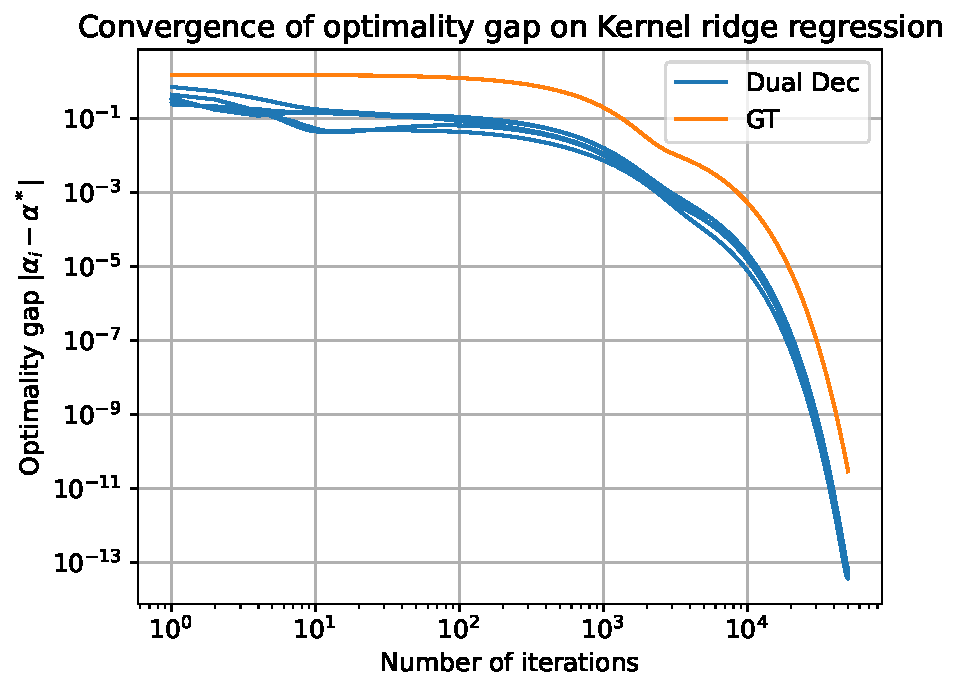
\includegraphics[width=12cm]{plot_background_Dual Dec vs GT.pdf}};
    \begin{scope}[x={(image.south east)}, y={(image.north west)}]
        
        % Graphe d'adjacence A
        \node[anchor=south west] at (0.15, 0.18) {
            \begin{tikzpicture}[scale=0.8, every node/.style={circle, fill=black, inner sep=1.2pt}]
                % Calcul automatique des positions des noeuds en cercle
                \foreach \i in {1,...,5}{
                    \node (n\i) at ({360/5 * \i}:1cm) {};
                }
                % Dessin des arretes si A[i,j] > 0
                \draw (n1) -- (n2); \draw (n1) -- (n3); \draw (n1) -- (n4); \draw (n1) -- (n5); \draw (n2) -- (n3); \draw (n2) -- (n4); \draw (n2) -- (n5); \draw (n3) -- (n4); \draw (n3) -- (n5); \draw (n4) -- (n5); 
            \end{tikzpicture}
        };

        % Matrice W dynamique
        \node[anchor=south] at (0.52, 0.2) {
            $I = \begin{bmatrix} 
            1 & -1 & 0 & 0 & 0 \\
            1 & 0 & -1 & 0 & 0 \\
            1 & 0 & 0 & -1 & 0 \\
            1 & 0 & 0 & 0 & -1 \\
            0 & 1 & -1 & 0 & 0 \\
            0 & 1 & 0 & -1 & 0 \\
            0 & 1 & 0 & 0 & -1 \\
            0 & 0 & 1 & -1 & 0 \\
            0 & 0 & 1 & 0 & -1 \\
            0 & 0 & 0 & 1 & -1
            \end{bmatrix}$
        };

        % Step-size lr dynamique
        \node[anchor=south west] at (0.75, 0.25) {
            $s = 0.01$
        };
    \end{scope}
\end{tikzpicture}
\end{document}
